\documentclass[xcolor=svgnames,handout]{beamer}

\usepackage[utf8x]    {inputenc}
\usepackage[T1]      {fontenc}
\usepackage[english] {babel}

\usepackage{multicol} % Pra colocar o TOC em duas colunas

\usepackage{amsmath,amsfonts,graphicx}
\usepackage{beamerleanprogress}

%------------------------------------------------
\usepackage{lmodern} % Default font: latin modern font
%\usepackage{fourier} % Alternative font: utopia
%\usepackage{charter} % Alternative font: low-resolution roman font
\usepackage{tikz} % Required for colored boxes
\usepackage{booktabs} % Required for horizontal rules in tables
\usepackage{multicol} % Required for creating multiple columns in slides
\usepackage{microtype} % Better typography
%------------------------------------------------

%------------------------------------------------
%\usetocstyle{nodotnopagenumber}

%\AtBeginDocument{\renewcaptionname{english}{\contentsname}{\Large Fases}} % Change the name of the table of contents
%------------------------------------------------

%------------------------------------------------

%----------------------------------------------------------------------------------------
%	PRESENTATION INFORMATION
%----------------------------------------------------------------------------------------
\title
  [SNES\hspace{2em}]
  {Organização de Vídeo Games\\SNES}

\author
  [Alessandro Palmeira, João M. M. da Silva]
  {Alessandro Palmeira \space\space\space\space\space\space\space\space\space\space 6850476 \\João Marco Maciel da Silva \space 7577598}

\date
  {\today}

\institute
  {Organização de Computadores - MAC0412\\Instituto de Matemática e Estatística}

%----------------------------------------------------------------------------------------
%\makeatletter
%\newtocstyle[noonewithdot]{nodotnopagenumber}{\settocfeature{pagenumberbox}{\@gobble}}
%\makeatother
%\usetocstyle{nodotnopagenumber}

%\AtBeginDocument{\renewcaptionname{english}{\contentsname}{\Large Fases}} % Change the name of the table of contents

\begin{document}
\maketitle
%	TABLE OF CONTENTS
%----------------------------------------------------------------------------------------


\begin{frame}{Índice}
\begin{multicols}{2}
  \tableofcontents
  \end{multicols}

\end{frame}

%----------------------------------------------------------------------------------------
%	PRESENTATION SLIDES
%----------------------------------------------------------------------------------------



%------------------------------------------------

\begin{frame}{História dos Vídeo Games}
\section{Visão Geral}
\subsection{História dos Vídeo Games}
\begin{itemize}
	\item Primórdios
	\begin{itemize}
		\item 1958 - "Tennis For Two".\pause
		\begin{figure}[t]
		    \centering
		    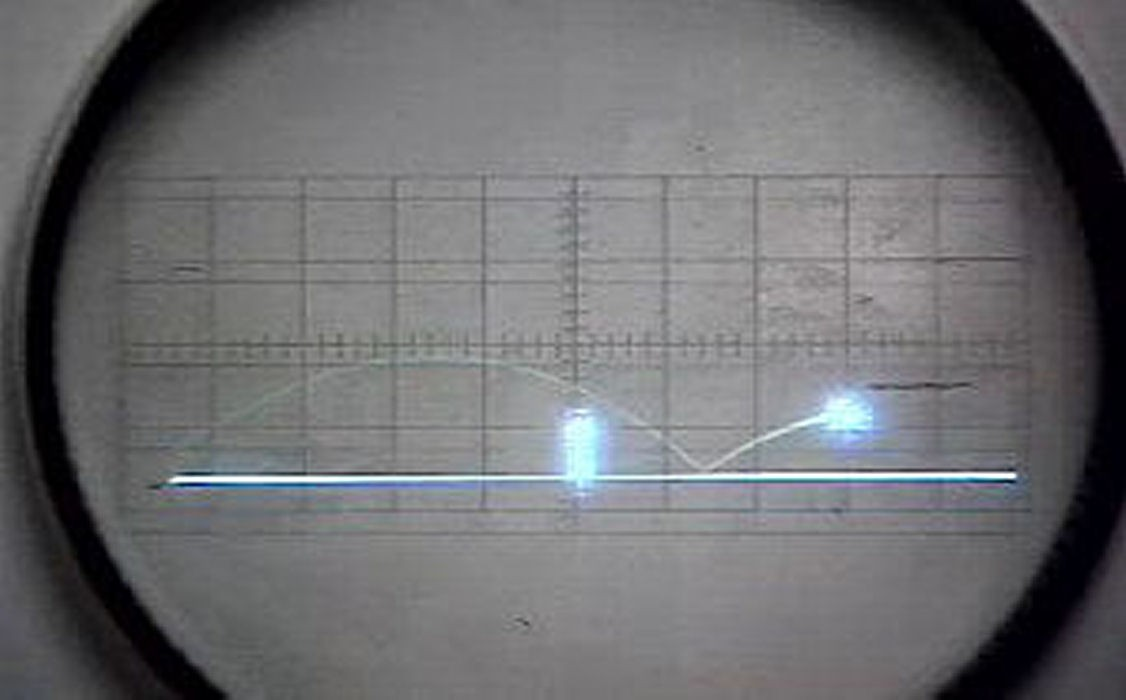
\includegraphics[scale=0.07]{imagens/tennis-for-two}
		  \end{figure}\pause
		\item 1962 - primeiro jogo em computadores dotados de transistores - "SpaceWar!"\pause
				\begin{figure}[t]
				    \centering
				    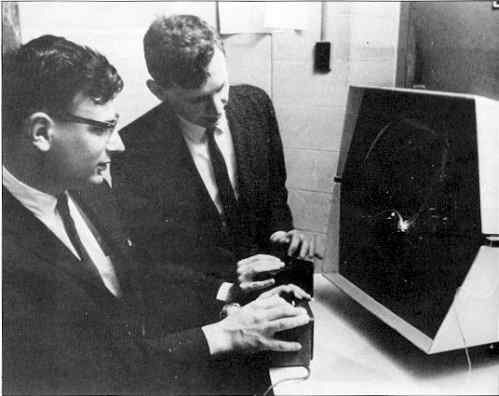
\includegraphics[scale=0.2]{imagens/golden_age3}
				  \end{figure}\pause
	\end{itemize}
\end{itemize}

\end{frame}

\begin{frame}{História dos Vídeo Games}
\begin{itemize}
	\item Primeira Geração(1972 - 1977)
	\begin{itemize}
	\item 1971 - Galaxy Game and Computer Space\pause
	\item 1972 - Odyssey 100 - primeiro vídeo game doméstico\pause
	\item 1972 - Fundação da Atari - Pong\pause
	\item 1976 - Fairchild Channel F - primeiro video game programável\pause
	\item 1977 - GunFight - primeiro jogo a usar microprocessadores\pause
	\item 1977 - crise dos Vídeo Games, só sobrevivem no mercado Atari e Magnavox\pause
	\end{itemize}
	\begin{figure}[t]
    \centering
	    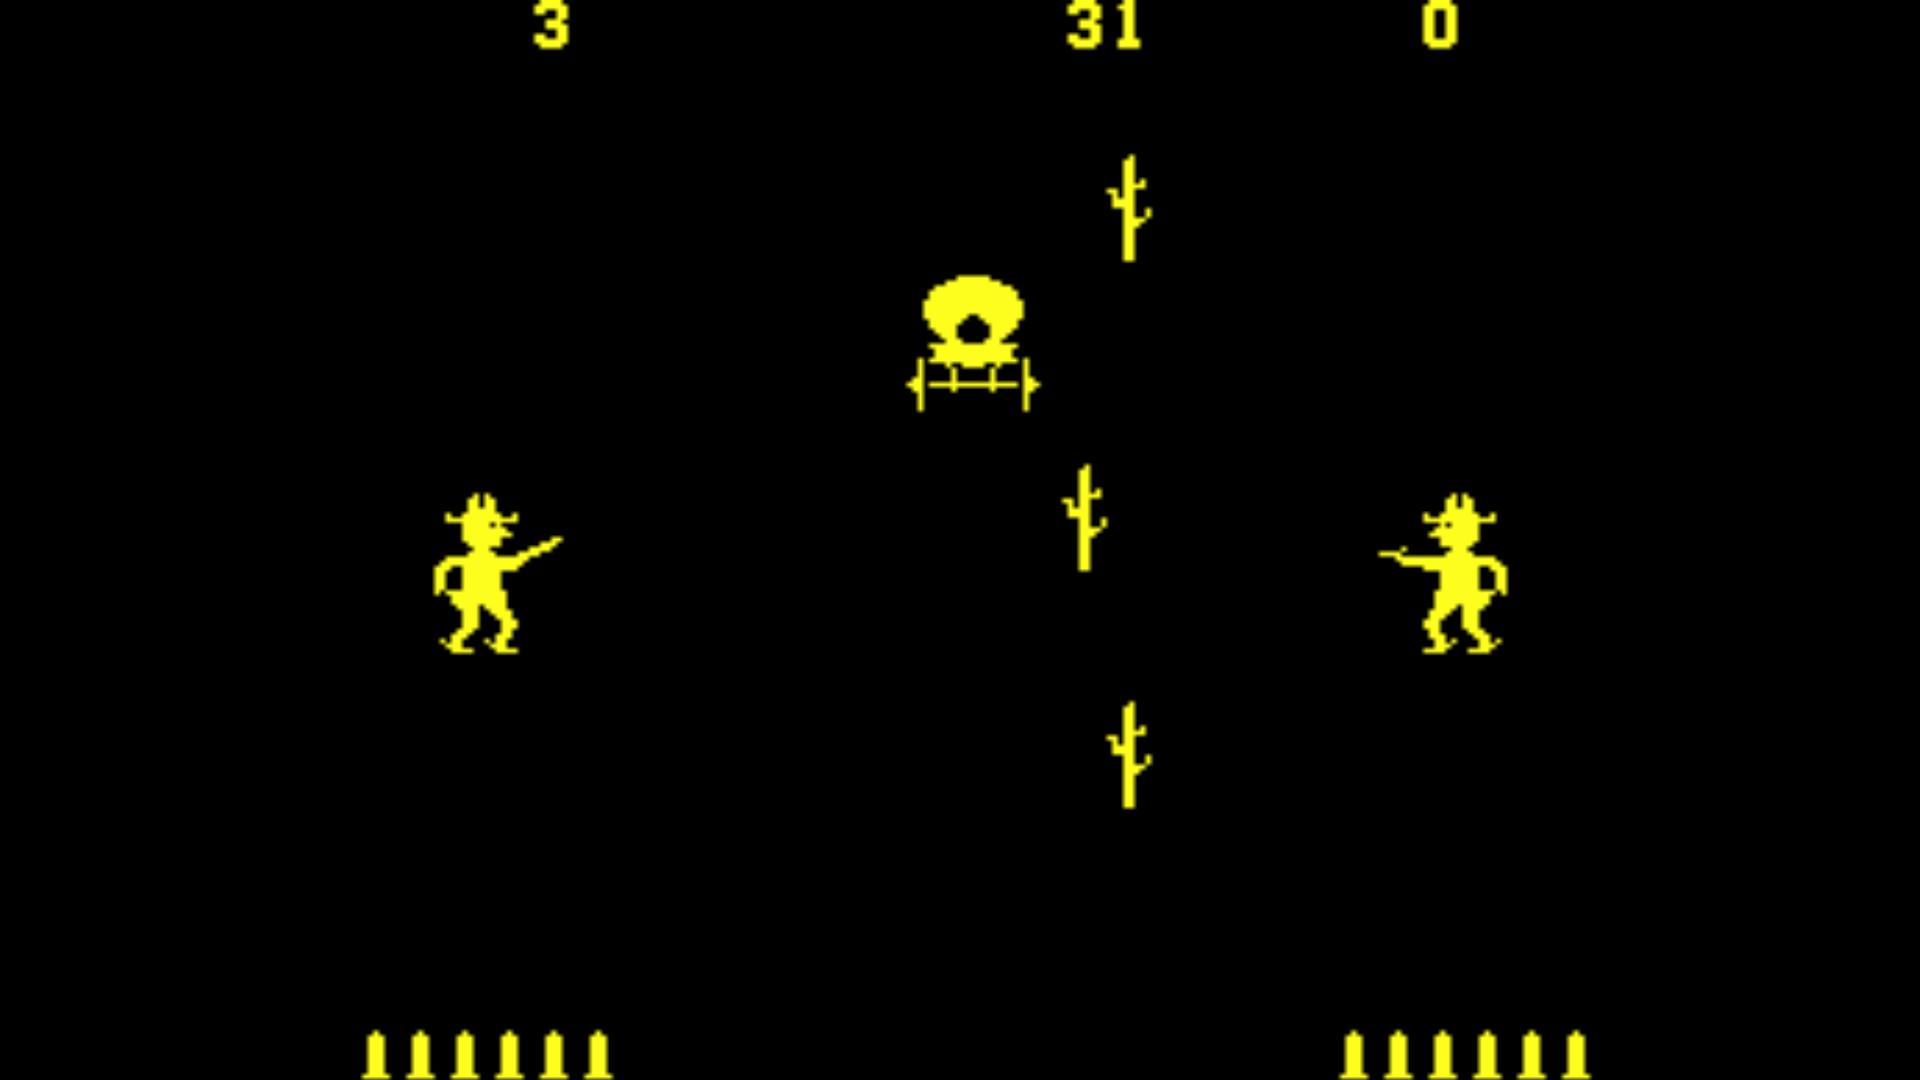
\includegraphics[scale=0.1]{imagens/gunfight}
	\end{figure}
\end{itemize}
\end{frame}
%------------------------------------------------

\begin{frame}{História dos Vídeo Games}
\begin{itemize}
	\item Segunda Geração(1977 - 1983)\pause
	\begin{itemize}
	\item 1977 - Atari 2600 - primeiro grande sucesso de vendas de consoles domésticos\pause
	\item 1978 - Nintendo entra no mercado de games\pause
	\item 1978 - Space Invaders para arcade provoca falta de moedas no mercado japonês\pause
	\item 1979 - Lunar Lander, primeiro jogo comercial com gráficos vetoriais.\pause
	\item 1979 - Sega entra para o mercado de vídeo games\pause
	\item 1980 - Pac-man\pause
	\item 1981 - Donkey Kong e Jumpman (Mario)\pause
	\item 1981 - Primeira pessoa a morrer jogando vídeo game(e não era chinês)\pause
	\item 1981 - Jogos Arcade rendem US\$5Bi\pause
	\item 1983 e 1984 - Segunda crise dos Vídeo Games
	\end{itemize}
		\begin{figure}[t]
	    \centering
		    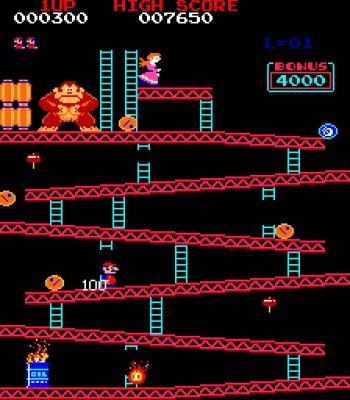
\includegraphics[scale=0.1]{imagens/mario}
		\end{figure}
\end{itemize}
\end{frame}

\begin{frame}{História dos Vídeo Games}
\begin{itemize}
	\item Terceira Geração(1983 - 1995)(8-bit)\pause
	\begin{itemize}
	\item 1984 - Nintendo lança o Famicom, primeiro vídeo game de sucesso com gamepad\pause
	\item 1985 - port do Super Mario Bros para Famicom\pause
	\item 1986 - Nintendo lança o Famicom nos EUA com o nome "NES"\pause
	\item 1986 - Master-System\pause
	\item 1986 - Vampire Killer(Precursor de Castlevania), The Legend of Zelda e Dragon Quest\pause
	\item 1987 - Final Fantasy e Metal Gear\pause
	\item 1988 - Fighting Street e Tetris\pause
	\item 1989 - Atari "desbloqueia" NES e lança jogos não autorizados
	\end{itemize}
		\begin{figure}[t]
	    \centering
		    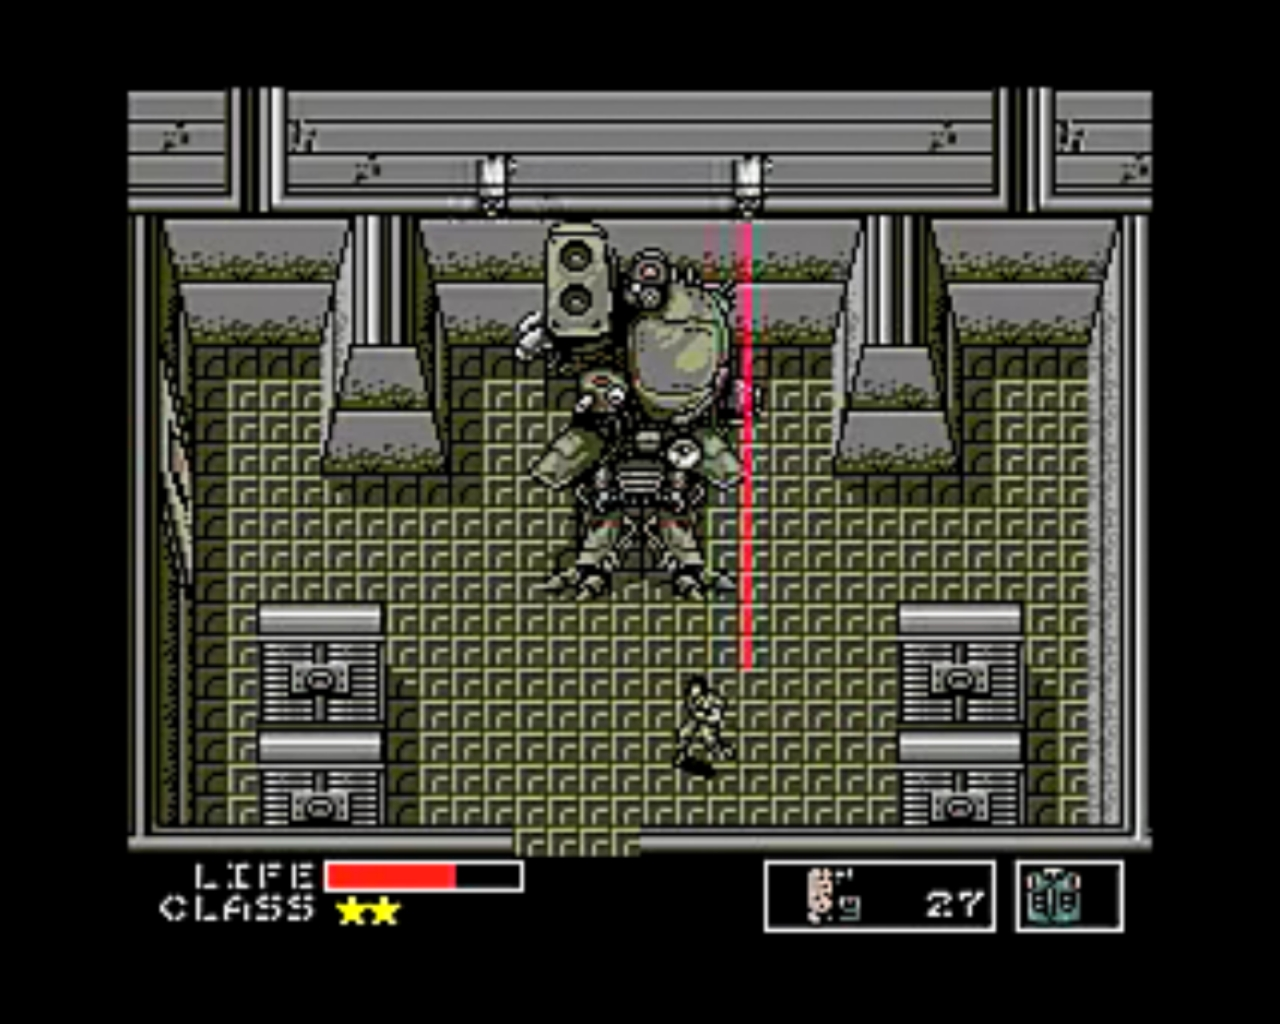
\includegraphics[scale=0.1]{imagens/metal-gear}
		\end{figure}
\end{itemize}
\end{frame}

\begin{frame}{História dos Vídeo Games}
\begin{itemize}
	\item Quarta Geração(1988 - 1999)(16-bit)\pause
	\begin{itemize}
	\item 1988 - Mega Drive/Genesis\pause
	\item 1990 - Super NES\pause
	\item 1992 - 3D básico por processadores adicionais inclusos nos cartuchos com resolução baixa e framerate < 4fps\pause
	
	\end{itemize}
		\end{itemize}
		\begin{figure}[t]
	    \centering
		    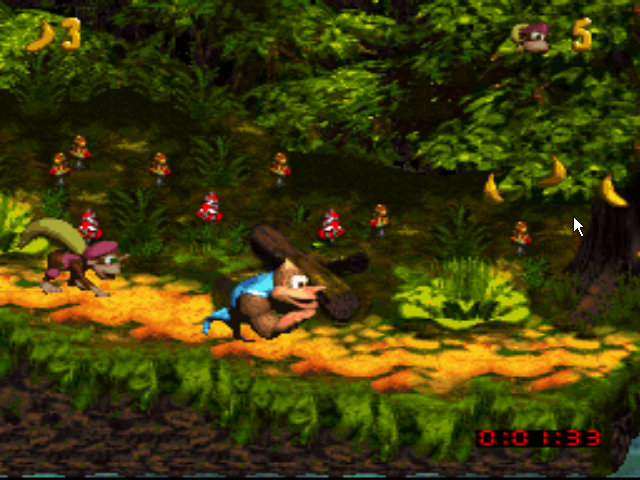
\includegraphics[scale=0.3]{imagens/dk3}
		\end{figure}
	\end{frame}
	
	\begin{frame}{História dos Vídeo Games}
		\begin{itemize}
	\item Quinta Geração(1993 - 2006)(32 e 64-bit)\pause
	\begin{itemize}
		\item Gráficos 3D, alguns Vídeo Games a CD\pause
		\item 1993 - Atari Jaguar\pause
		\item 1994 - Sega Saturn, Sony Playstation\pause
		\item 1996 - Nintendo 64\pause
		\item 1997 - Nokia lança Snake para seus celulares\pause
		\item 1998 - GameBoy\pause
		\item 2000 - China bane Vídeo Games do país\pause
		\end{itemize}
				\begin{figure}[t]
			    \centering
				    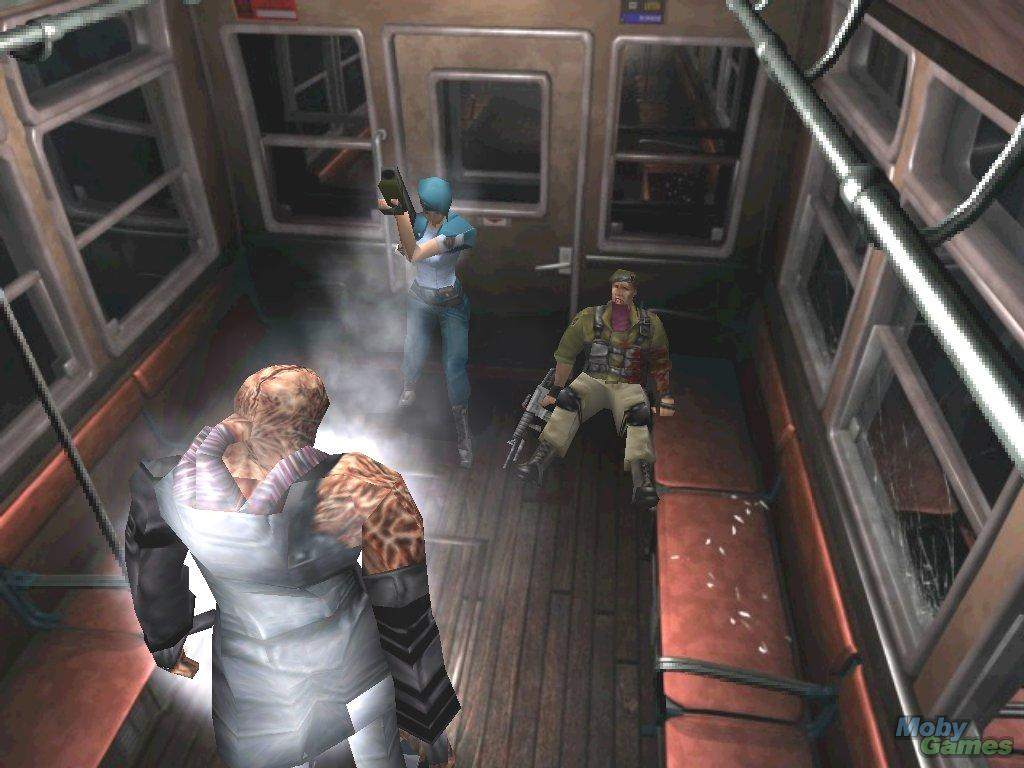
\includegraphics[scale=0.15]{imagens/re3}
				\end{figure}
\end{itemize}
\end{frame}

\begin{frame}{História dos Vídeo Games}
\begin{itemize}
	\item Sexta Geração(1998 - 2013)\pause
	\begin{itemize}
	\item abandono do mercado brasileiro\pause
	\item emuladores de plataformas antigas ganham força\pause
	\item crescimento do mercado de jogos online\pause
	\item DVD aparece como mídia\pause
	\item retorno de controles diferentes do joypad, como joystics, armas e tapetes de dança\pause
	\item 1998 - Dreamcast\pause
	\item 2000 - Playstation 2\pause
	\item 2001 - GameCube\pause
	\item 2001 - Microsoft entra no mercado de Vídeo Games - XBOX\pause
	\end{itemize}
\end{itemize}
		\begin{figure}[t]
	    \centering
		    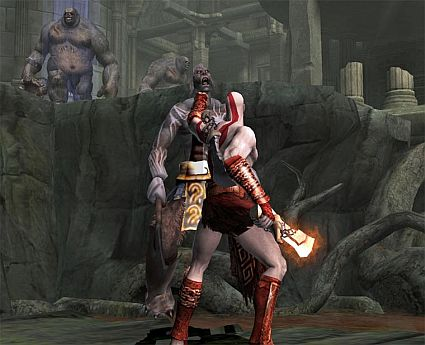
\includegraphics[scale=0.3]{imagens/gow2}
		\end{figure}
\end{frame}

\begin{frame}{História dos Vídeo Games}
\begin{itemize}
	\item Setima Geração(2005 - presente)\pause
	\begin{itemize}
		\item 3D chega aos portáteis no DS e PSP\pause
		\item Blu-Ray e HD-DVD surgem como mídia para jogos\pause
		\item Armazenamento em HD nos Vídeo Games\pause
		\item consoles com jogos online\pause
		\item O corpo se torna um novo controle(wii, ps Move e MS Kinect) e revoluciona Gameplay\pause
		\item Brasil volta ao Mercado de Jogos\pause
		\item Uso de Vídeo Games para computação de alto desempenho(PS3)\pause
		\item 2005 - XBOX 360\pause
		\item 2006 - PS3 e Wii\pause
		\item 2010 - Microsoft Kinect\pause
		\end{itemize}
		\end{itemize}
				\begin{figure}[t]
			    \centering
				    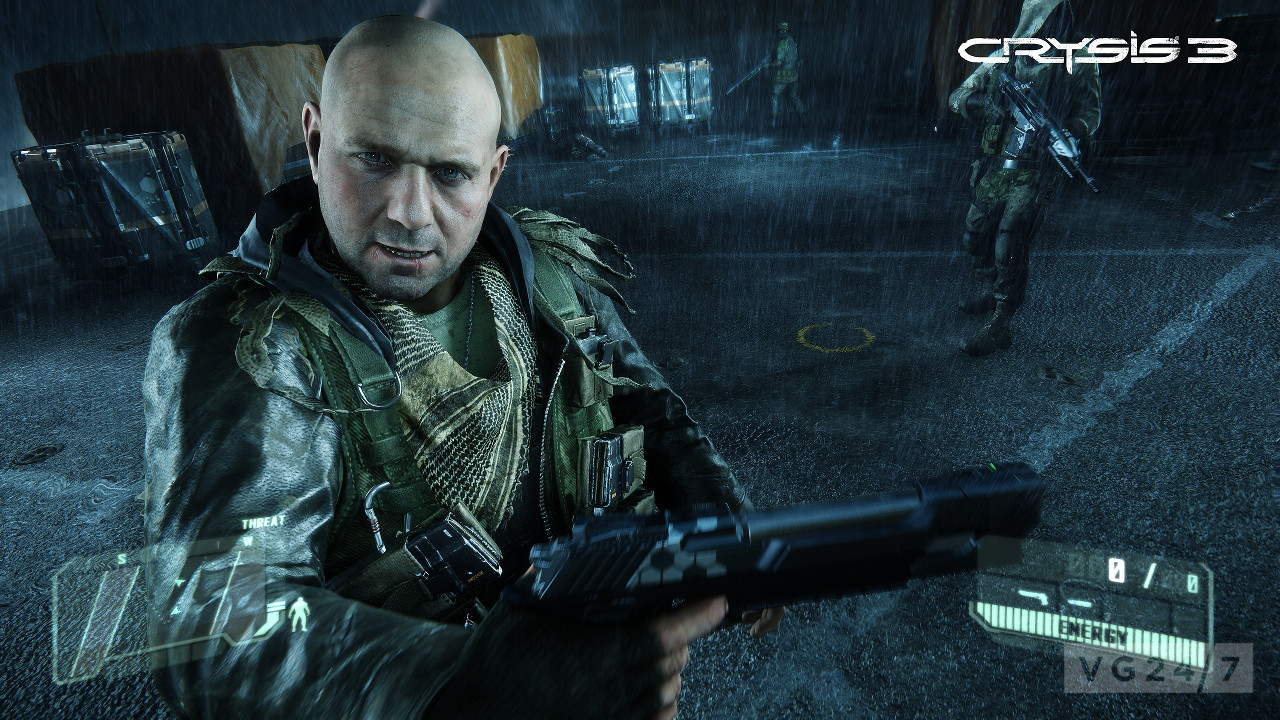
\includegraphics[scale=0.1]{imagens/c3}
				\end{figure}
\end{frame}

\begin{frame}{História dos Vídeo Games}
\begin{itemize}

	\item Oitava Geração(2012 - presente)\pause
	\begin{itemize}
		\item 2012 - WiiU\pause
		\item 2013 - XBOX One e PS4
	\end{itemize}
\end{itemize}
				\begin{figure}[t]
			    \centering
				    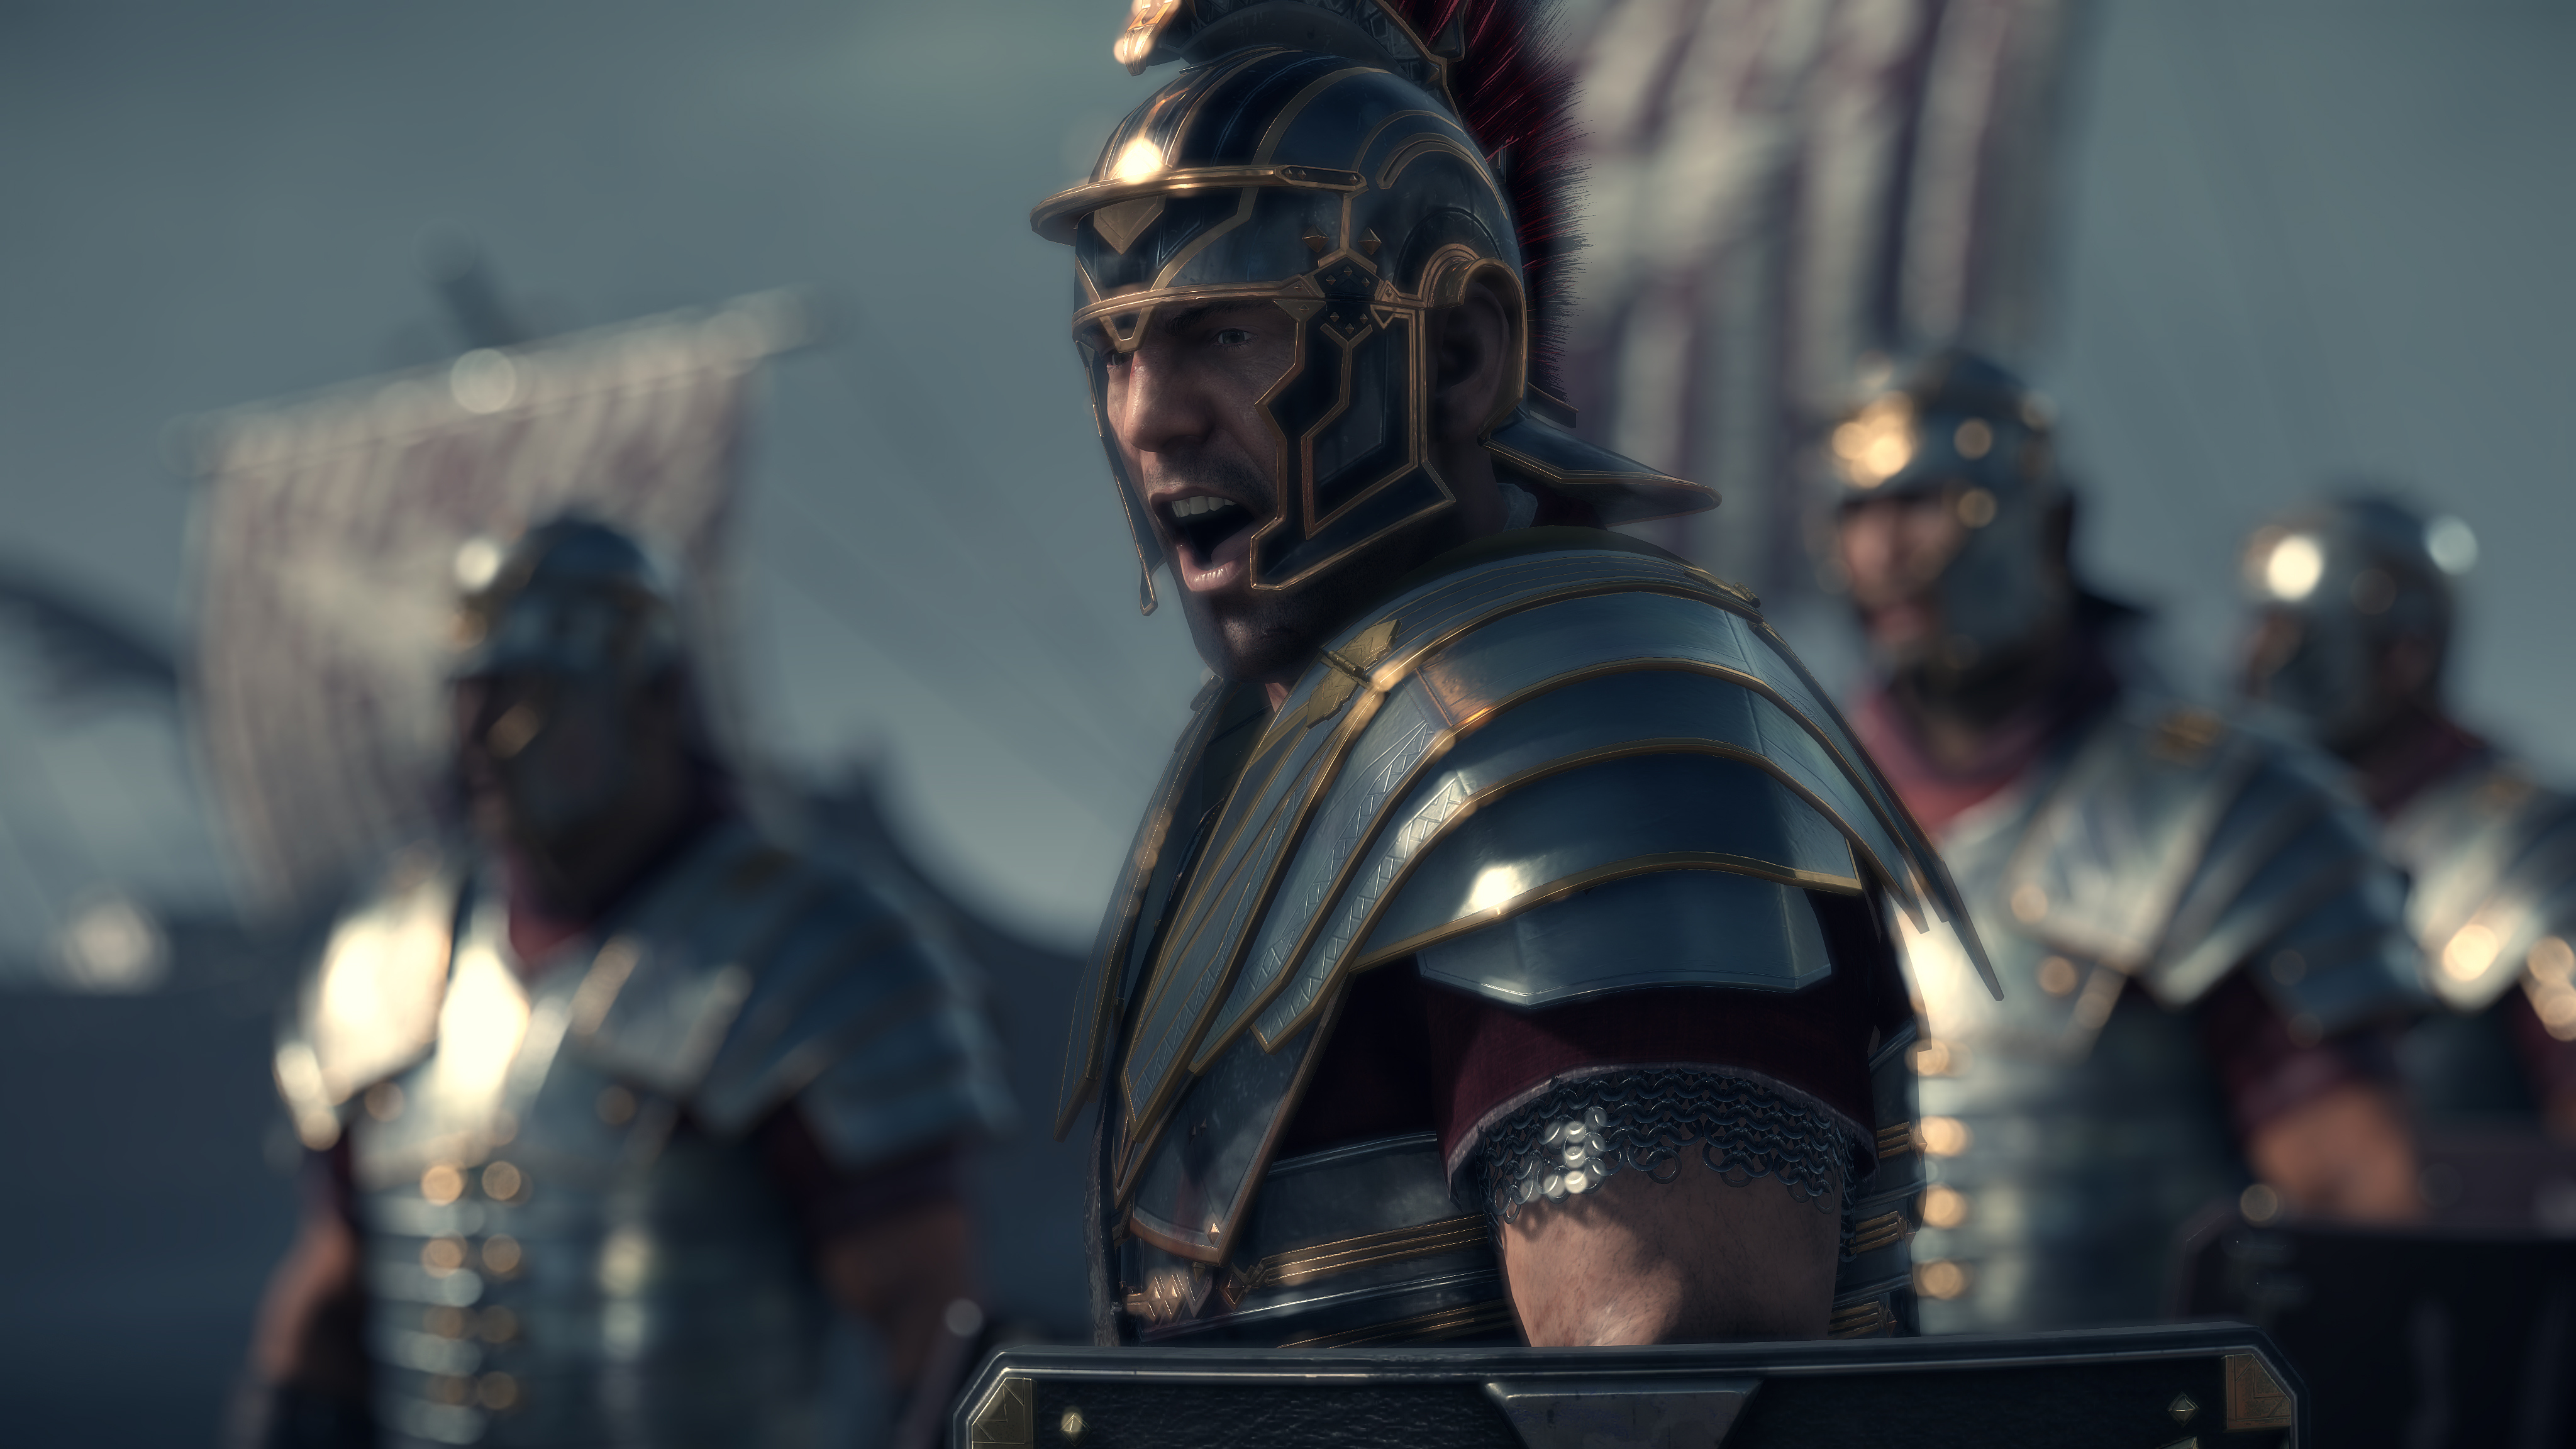
\includegraphics[scale=0.07]{imagens/ryse}
				\end{figure}
\end{frame}
%---
	
\begin{frame}{SNES}
\section{SNES}

\begin{figure}[t]
    \centering
    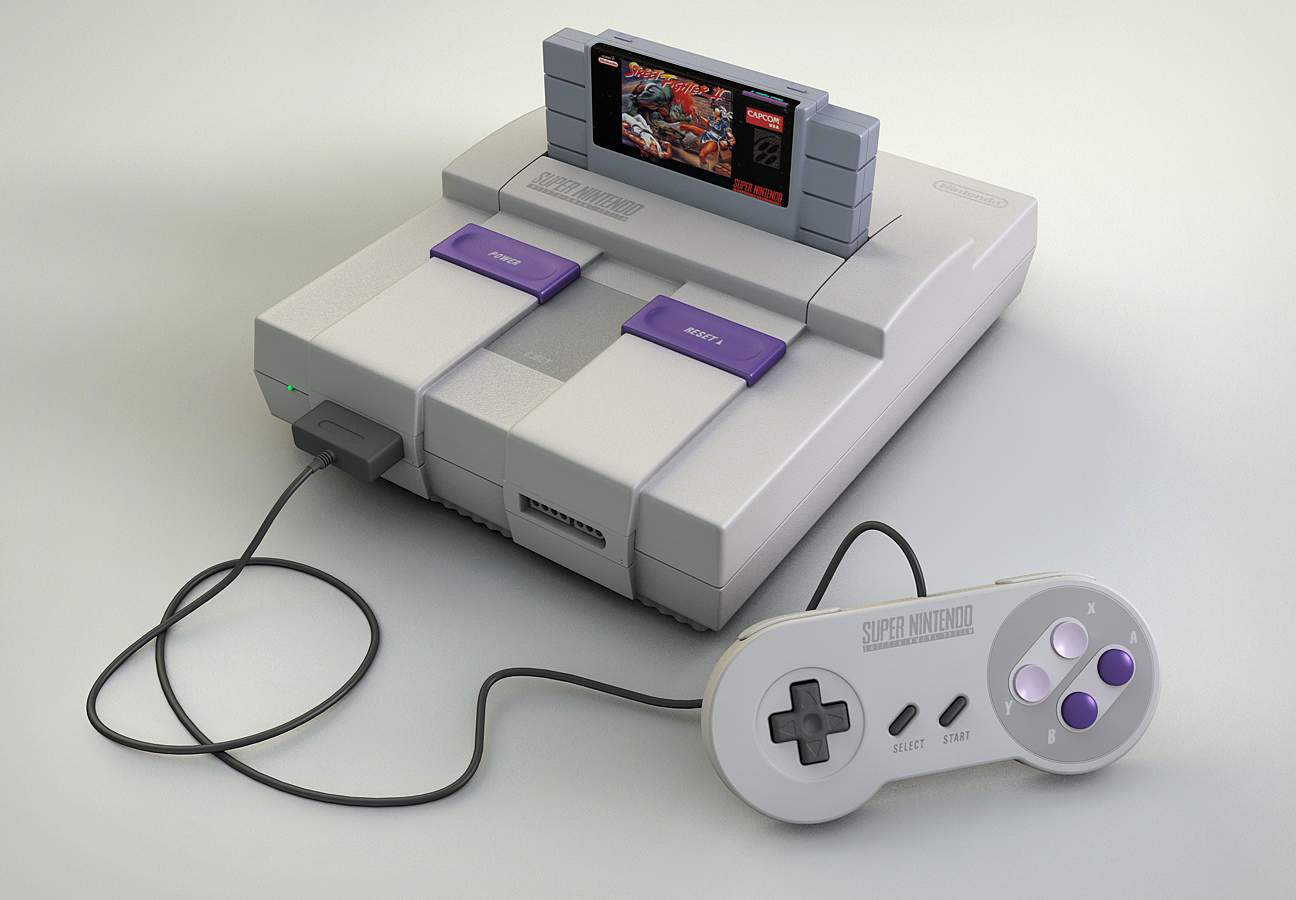
\includegraphics[scale=0.2]{imagens/snes}
\end{figure}
\end{frame}


%------------------------------------------------

\begin{frame}{Especificações Técnicas}
\subsection{Especificações Técnicas}

\begin{itemize}
  \item{Arquitetura 16-bits}
  \item{32768 $(2^{15})$ cores}
  \item{Som com 8 canais de alta qualidade (32kHz - 16 bit Stereo)}
\end{itemize}

\begin{figure}
  \begin{center}
    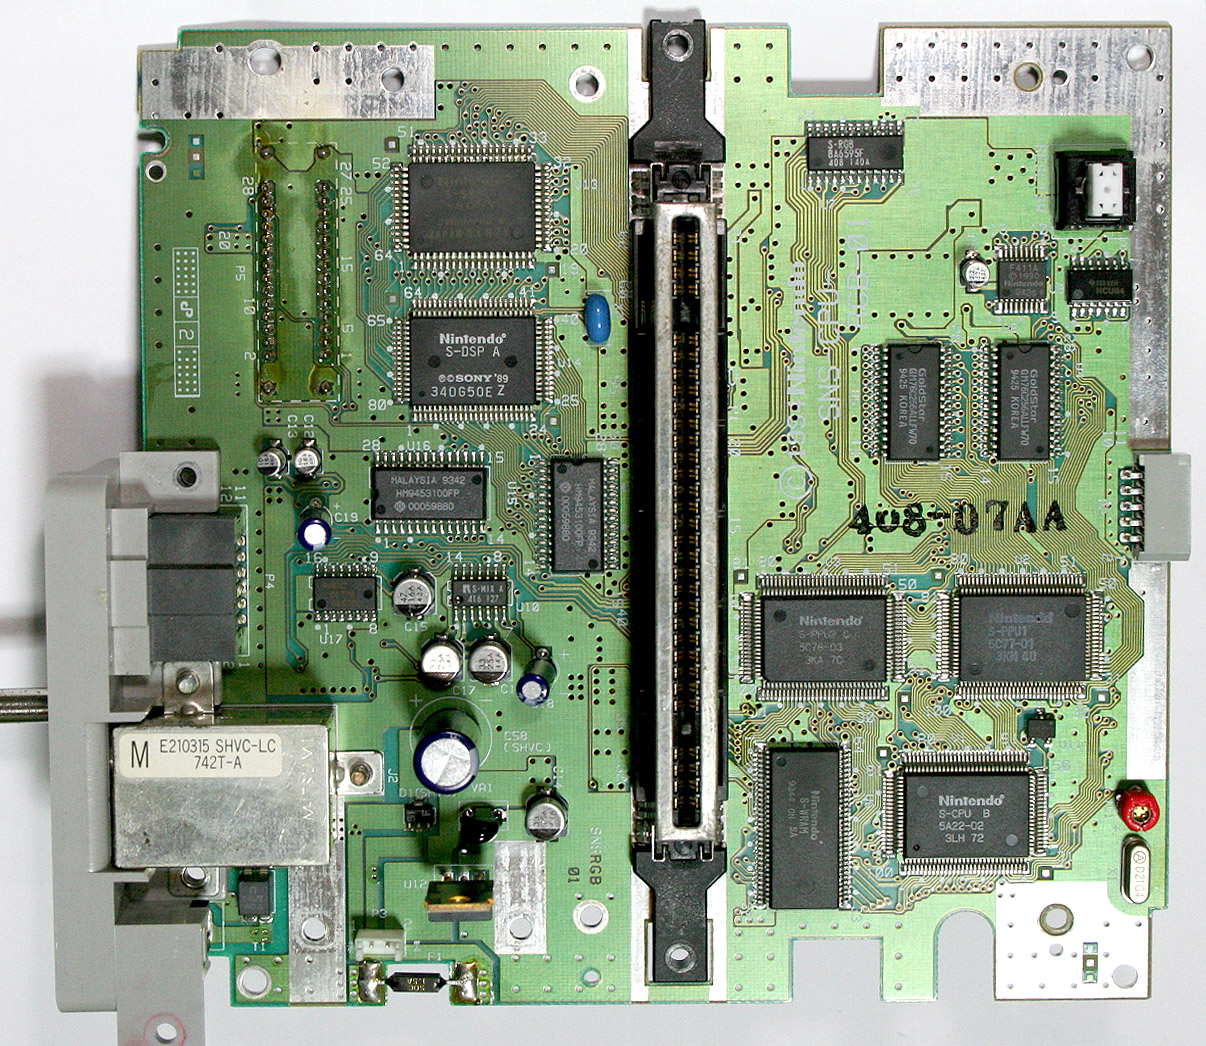
\includegraphics[height=5cm, width=\textwidth, keepaspectratio]{SNES-CPU-RGB01_01.jpg}
    \label{fig:}
    \caption{Placa-Mãe do SNES}
  \end{center}
\end{figure}

\end{frame}

%------------------------------------------------

\begin{frame}{CPU}
\section{A CPU}
  \begin{itemize}
    \item{Chip customizado da Nintendo baseado no microprocessador 65c816}
    \item{Clock 21.47727 MHz (NTSC)/ 21.28137 MHz (PAL) divididos em 6, 8 ou 12.}
    \begin{itemize}
      \item{6:  Acessos gerais}
      \item{8:  Acesso a WRAM}
      \item{12: Acesso aos controles}
    \end{itemize}
    \item{Barramento de dados de 8-bit, controlado por 2 barramentos de endereços:}
    \begin{itemize}
      \item{Bus "A" (24-bit): Acesso geral}
      \item{Bus "B" (8-bit): Suporte aos processadores de áudio e vídeo.}
    \end{itemize}
    \item{Usa DMA (Direct Access Memory) para atingir até 2.68 MB/s de transferência de dados.}
  \end{itemize}
\end{frame}

%------------------------------------------------

\begin{frame}{Vídeo}
\section{O Vídeo}
    \begin{itemize}
      \item{64kB de SRAM}
      \item{544bytes de OAM (Object Attribute Memory) para armazenar sprites}
      \item{256x15 bits de CGRAM (Color Generator RAM) para a paleta de cor}
      \item{Diferentes resoluções PAL/NTSC e Progressivo/Entrelaçado}
      \begin{itemize}
        \item{Progressivo: 256 × 224, 512 × 224, 256 × 239, 512 × 239}
        \item{Entrelaçado: 512 × 448, 512 × 478}
      \end{itemize}
      \item{Pixel Depth: Indexado e direto}
    \end{itemize}
\end{frame}

\begin{frame}{Vídeo}
    \begin{itemize}
      \item{Diferentes modos com resolução, número de camadas e esquema de cores diferentes}
      \begin{itemize}
        \item{Modo 7 suporta rotação e dilatação de camadas usando transformações de matrizes}
      \end{itemize}
    \end{itemize}
  \begin{figure}
  \begin{center}
    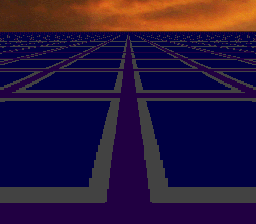
\includegraphics[height=4.5cm, width=\textwidth, keepaspectratio]{Mode_7.png}
    \label{fig:}
    \caption{Modo 7}
  \end{center}
\end{figure}
\end{frame}

%------------------------------------------------

\begin{frame}{Áudio}
\section{O Áudio}
\begin{itemize}
  \item{8-bit Sony SCP700, 16-bit DSP (Processador de Sinal Digital)}
  \item{64kB dse SRAM compartilhada e 64 bytes de Boot ROM}
  \item{Clock: 24.576 MHz}
  \item{Praticamente independente do resto do sistema}
  \item{Comunicação com a CPU é feita apenas via 4 registradores do Bus B}
  \item{Acesso à RAM multiplexado entre o SCP700(1/3) e o DSP(2/3)}
  \item{O SPC700 roda programas carregados pela Boot ROM e aceita instruções e dados da CPU para manipular o DSP e gerar o áudio}
\end{itemize}
\end{frame}

%------------------------------------------------

\begin{frame}{Cartucho}
\section{Cartucho}
\begin{itemize}
	\item Snes pode endereçar 128Mbit, apenas 117Mbit para uso do cartucho\pause
	\item Um cartucho contem em geral 95Mbit de espaço para ROM mais 8Mbit saves\pause
	\item Apesar do espaço, os maiores jogos ocupavam 48Mbit\pause
	\item Os saves são guardados em capacitores, e mantidos à bateria\pause
	\item Máximo de 62 pinos, a um clock de 21,477 MHz
\end{itemize}
\begin{figure}
  \begin{center}
    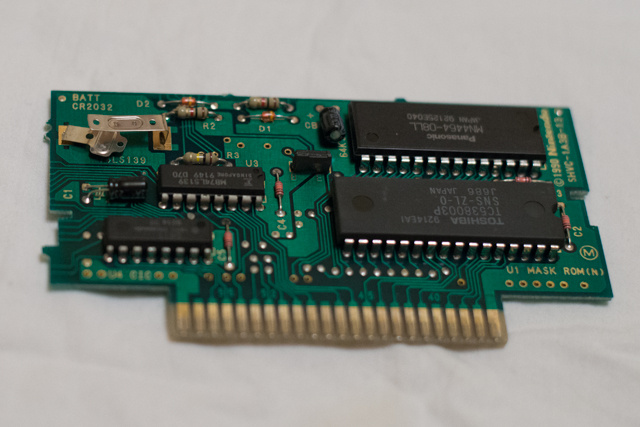
\includegraphics[height=4cm, width=\textwidth, keepaspectratio]{imagens/cartucho}
    \label{fig:}
  \end{center}
\end{figure}
\end{frame}

\begin{frame}{Enhancement Chips}
\subsection{Enhancement Chips}
\begin{itemize}
  \item{Plano: Evitar que a CPU fosse complexa e cara e ficasse obsoleta em pouco tempo}
  \item{Design: Co-processadores podiam ser adicionados no cartucho, e a interface era feita utilizando mais pinos}
\end{itemize}
\begin{figure}
  \begin{center}
    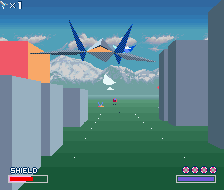
\includegraphics[height=4cm, width=\textwidth, keepaspectratio]{SNES_Star_Fox.png}
    \label{fig:}
    \caption{Star Fox utilizando o chip Super FX}
  \end{center}
\end{figure}
\end{frame}

\begin{frame}{CIC e Pirataria}
\section{CIC e Pirataria}
\begin{itemize}
\item Composto por um microcontrolador no console que checa ao cartucho inserido para autenticação.
\item Enquanto o cartucho não responder ou responder errado então o CIC reseta a CPU a cada ciclo.
\item O reinício constante da CPU impedia o console de ser inicializado.
\end{itemize}
\begin{figure}
  \begin{center}
    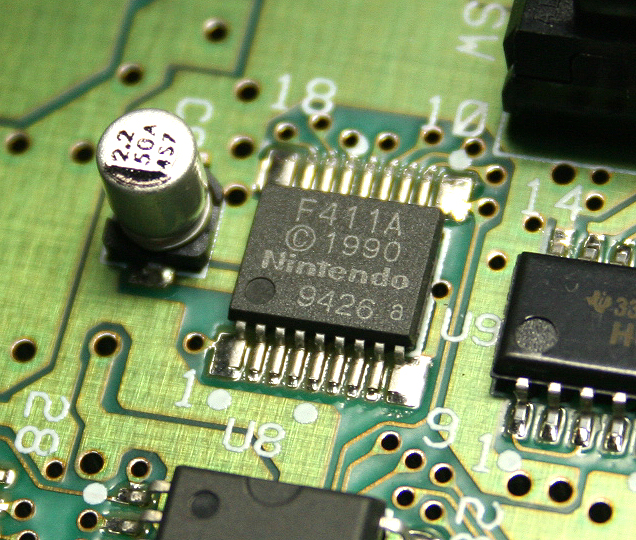
\includegraphics[height=4.7cm, width=\textwidth, keepaspectratio]{imagens/cic}
    \label{fig:}
  \end{center}
\end{figure}
\end{frame}
%------------------------------------------------

\begin{frame}{Mão na massa}
\section{Mão na massa}
\begin{itemize}
  \item{Como era feita a programação?}
  \item{Código simples que inicializa o console e muda a cor de fundo}
  \item{Código da trilha sonora do Top Gear}
  \item{Código mais complexo - Jogo da Velha}
\end{itemize}
\end{frame}

%------------------------------------------------

\begin{frame}{Conclusões}
\section{Conclusões}
\begin{itemize}
  \item{O SNES é muito mais complexo do que parece}
  \item{A documentação é toda não-oficial e só muito recentemente (últimos 5 anos) vem sendo organizada}
  \item{É uma pena que a documentação oficial, desde os datasheets dos componentes até o código fonte em ASM dos jogos, nunca foi publicada.}
  \item{O estudo do console deu uma ótima visão de como todos os componentes funcionam em conjunto}
  \item{O estudo dos códigos em Assembly mostrou vários aspectos práticos interessantes, como a ausência de frameworks e até aspectos bastante técnicos, como o V-Blank}
\end{itemize}

\end{frame}
%------------------------------------------------

\begin{frame}{Referências}
\begin{itemize}
\item História dos Vídeo Games:
\begin{itemize}	
\item http://en.wikipedia.org/wiki/History\_of\_video\_games
\end{itemize}
\item Hardware geral:
\begin{itemize}	
\item 	http://www.caitsith2.com/snes/
\item 	http://digitalfantasy.angelfire.com/snes-hardware-specifications.html
\item 	http://en.wikipedia.org/wiki/Super\_Nintendo\_Entertainment\\\_System\_technical\_specifications
\item 	http://de.academic.ru/dic.nsf/dewiki/1219157
\item 	http://pikensoft.com/old/docs/SNES\_chip\_labels.txt
\item 	http://nocash.emubase.de/fullsnes.txt
\end{itemize}
\end{itemize}
\end{frame}

\begin{frame}{Referências}
\begin{itemize}
\item Áudio:
\begin{itemize}	
\item 	http://en.wikipedia.org/wiki/Nintendo\_S-SMP
\item 	http://snesmusic.org/v2
\item 	http://snesmusic.org/files/spc700.html
\item 	http://web.archive.org/web/20090106230547/http://www.a\\lpha-ii.com/snesmusic/files/spc700\_apu\_manual.txt
\end{itemize}
\item Processador:
\begin{itemize}	
\item 	http://en.wikipedia.org/wiki/WDC\_65816/65802
\item 		http://westerndesigncenter.com/wdc/docume\\ntation/w65c816s.pdf
\item 	http://en.wikibooks.org/wiki/6502\_Assembly
\end{itemize}
\item Programação:
\begin{itemize}	
\item 	http://en.wikibooks.org/wiki/Super\_NES\_Programming
\item 	http://wiki.superfamicom.org/snes/show/HomePage
\end{itemize}
\end{itemize}
\end{frame}

\begin{frame}{Referências}
\begin{itemize}
\item ROM Hacking:
\begin{itemize}	
\item 	http://www.romhacking.net
\item 	http://www.romhacking.net/start/
\end{itemize}
\item Controle:
\begin{itemize}	
\item www.gamesx.com/controldata/snesdat.htm
\end{itemize}
\item CIC:
\begin{itemize}	
\item en.wikipedia.org/wiki/CIC\_(Nintendo)
\end{itemize}
\item Cartucho:
\begin{itemize}
\item http://motherboard.vice.com/blog/pictures-how-to-replace-an-snes-cartridge-save-game-battery
\item http://www.caitsith2.com/snes/flashcart/cart-chip-pinouts.html
\end{itemize}
\end{itemize}

\end{frame}

\begin{frame}{Dúvidas}
	\begin{itemize}
	\item Dúvidas?
	\end{itemize}
\end{frame}

%------------------------------------------------

%----------------------------------------------------------------------------------------

\end{document}
